\documentclass{beamer}
\usepackage[utf8]{inputenc}
\usepackage{ngerman}
\usepackage{graphicx}

\usetheme{Warsaw}
\useinnertheme{circles}
\useoutertheme{smoothbars}
\setbeamercovered{transparent}

\title{Computer Vision Algorithmen auf einem DSP}
\titlegraphic{
\includegraphics[width=1.5cm]{img/TUG}}
\author{Thomas Ebner, Stefan Nöhmer}
\date{15.06.2011}


\begin{document}

	\frame{\titlepage}
	
% ============================= Stefan Part ================================
	
	\section{Einleitung}
	\begin{frame}{Einleitung}
	  
	  \begin{block}{\textbf{Hardware}}
	    BeagleBoard-xM
	    
      \texttt{www.beagleboard.org}
      
      TI OMAP Prozessor: ARM CPU, GPU, DSP
    \end{block}
    
    \begin{block}{\textbf{Algorithmen}}
      Computer Vision Algorithmen zur Featureerkennung
      
      \begin{itemize}
        \item \emph{Harris Corner Detector}
        \item \emph{SIFT}
      \end{itemize}
    \end{block}

  \end{frame}
	
	
	\section{Hardware}
		
		\subsection{BeagleBoard-xM}
		\begin{frame}{BeagleBoard-xM Übersicht}
			\begin{center}
        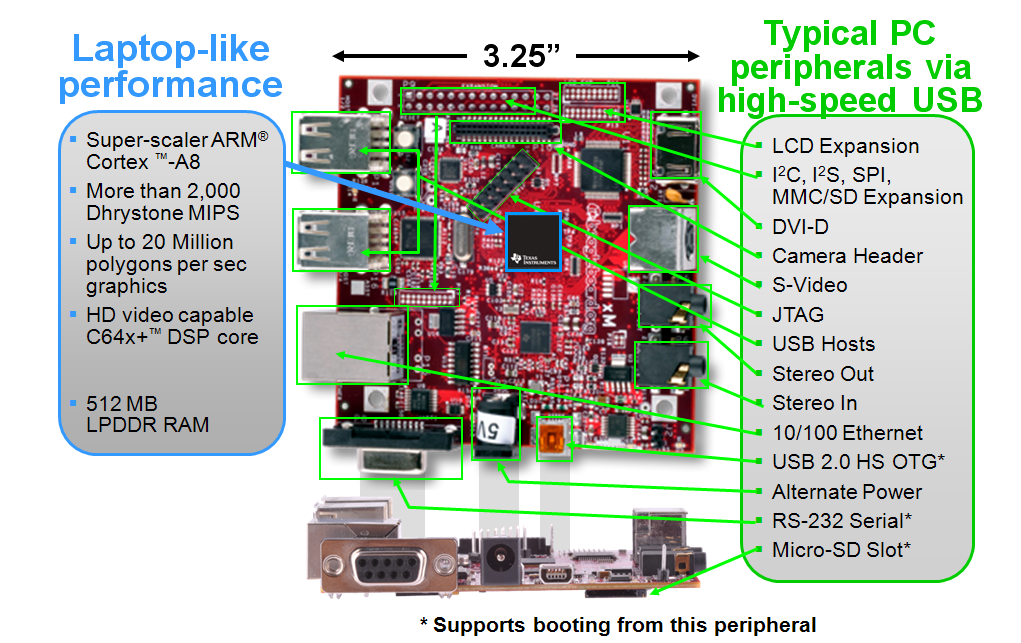
\includegraphics[height=0.7\paperheight]{./img/beagleboard-xm.png}
      \end{center}
		\end{frame}
		
		\begin{frame}{Verfügbare Ressourcen}
		  \begin{block}{TI OMAP}
		    \begin{itemize}
		      \item CPU: ARM Cortex-A8 (max. 1GHz)
		      \item Grafikbeschleuniger PowerSGX
		      \item Signalprozessor C64x+
		      \item 512MB RAM
		      \item Kamera mit 3MP
		    \end{itemize}
		  \end{block}
		  
		  \begin{block}{Software}
        \begin{itemize}
          \item Ubuntu Linux 11.04 für ARM
          \item spezielle Kernelmodule für TI OMAP
          \item Grafikbeschleunigung durch GPU
          \item Algorithmen auf DSP implementiert
        \end{itemize}
      \end{block}
		\end{frame}

		\subsection{TI OMAP Aufbau}
		\begin{frame}{TI OMAP Überblick}
		  \begin{center}
        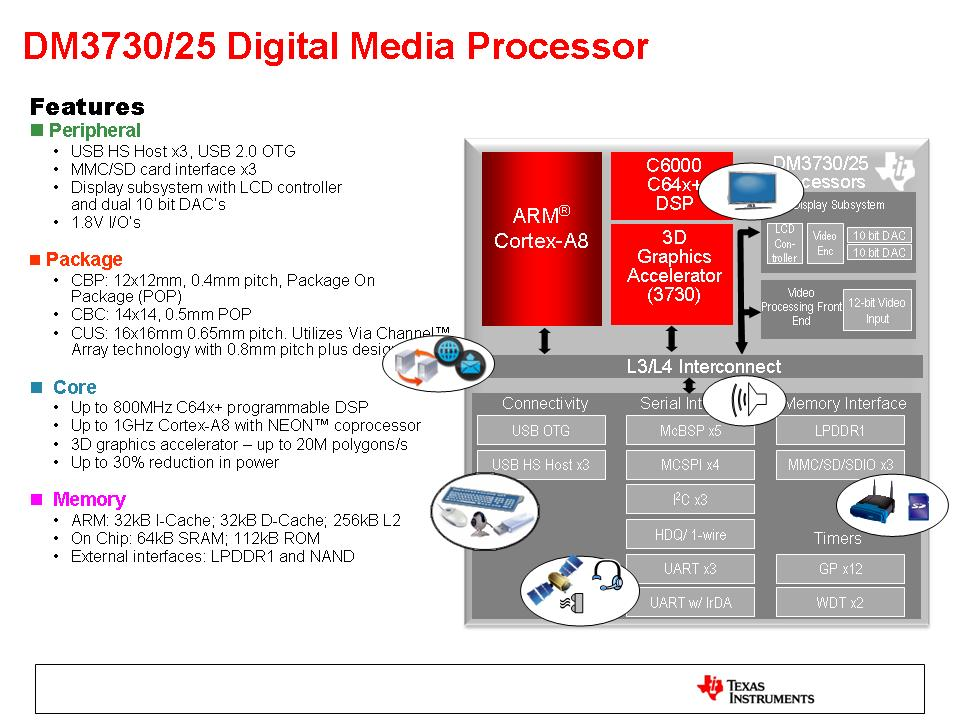
\includegraphics[height=0.7\paperheight]{./img/ti-omap.jpg}
      \end{center}
		\end{frame}
		
		\begin{frame}{TI OMAP Funktion}
		  \begin{block}{Eigenschaften des DSP}
		    \begin{itemize}
		      \item VLIW-Architektur
		      \item mehrere Funktionseinheiten:
		      \begin{itemize}
            \item Addierer
            \item Multiplizierer
            \item Bitweise Operationen
          \end{itemize}
		      \item schnelle, parallelisierbare Verarbeitung
		      \item ideal für Computer Vision Algorithmen
		      \item Beispiel: Faltung am DSP sehr effektiv
		    \end{itemize}
		  \end{block}
		  
		  \begin{block}{Kommunikation zur CPU}
	      \begin{itemize}
          \item Kontrollnachrichten via \emph{Mailboxes}
          \item Datenaustausch über Buffer im RAM
        \end{itemize}
      \end{block}
		\end{frame}
		
		\begin{frame}{Programmierung}
		  \begin{block}{CPU}
		    \begin{itemize}
          \item Standard-Compiler \texttt{arm-gcc}
		      \item in C/C++
		    \end{itemize}
		  \end{block}
		  
		  \begin{block}{DSP}
        \begin{itemize}
          \item spezieller VLIW-Compiler von TI
          \item in C/C++
          \item Compiler übernimmt Optimierung/Aufteilung
        \end{itemize}
      \end{block}
		\end{frame}
		
% =============================== Tom Part ==================================
		
  \section{Algorithmen}
    
    
  
				
		% --- Ende ---
		\begin{frame}
			\begin{center}
				\begin{large}
					Danke für die Aufmerksamkeit!
				\end{large}
			\end{center}
		\end{frame}

\end{document}
